\documentclass[10pt]{article}
\usepackage[T1]{fontenc}
\usepackage[utf8]{inputenc}
\usepackage{lmodern,microtype,amsmath,amssymb,booktabs,array,graphicx,float}
\usepackage[a4paper,margin=0.85in]{geometry}
\usepackage{fancyhdr}
\usepackage{placeins}
\usepackage[colorlinks=true,allcolors=blue]{hyperref}
\usepackage{url}
% Let tables flow across page boundaries without leaving large empty areas.
\renewcommand{\topfraction}{0.9}
\renewcommand{\bottomfraction}{0.8}
\renewcommand{\textfraction}{0.1}
\renewcommand{\floatpagefraction}{0.8}
\setcounter{topnumber}{3}
\setcounter{bottomnumber}{2}
\setcounter{totalnumber}{5}
\widowpenalty=10000
\clubpenalty=10000
\urlstyle{same}
\setlength{\parskip}{3pt}
\setlength{\intextsep}{8pt}
\setlength{\parindent}{0pt}
\setlength{\emergencystretch}{2em}
\setlength{\headheight}{14pt}
\pagestyle{fancy}
\fancyhf{}
\fancyhead[L]{VarBlockSpMM}
\fancyhead[R]{Cohen Brunner Thomas}
\fancyfoot[C]{\thepage}
\newcommand{\AuditCsr}{3.518}
\newcommand{\AuditGrouped}{4.769}
\newcommand{\AuditBsr}{0.834}
\newcommand{\AuditApplication}{0.296}
\newcommand{\AuditDefaultCsr}{5.656}
\newcommand{\AuditApplicationGrouped}{6.924}
\newcommand{\AuditApplicationGroupedLow}{6.020}
\newcommand{\AuditApplicationGroupedHigh}{7.851}
\newcommand{\AuditCompactSpeedup}{3.382}
\newcommand{\AuditCsrWins}{128}
\newcommand{\AuditGroupedWins}{128}
\newcommand{\AuditBsrWins}{9}
\newcommand{\AuditApplicationWins}{0}
\newcommand{\AuditBsrLosses}{23}
\newcommand{\AuditApplicationLosses}{12}

\newcommand{\NativeBsrRatio}{0.390}
\newcommand{\NativeStartupRatio}{3.953}
\newcommand{\NativeTenProductsRatio}{2.668}
\newcommand{\NativeCsrStorageRatio}{1.948}
\newcommand{\RhsEightUpgrade}{1.777}
\newcommand{\RhsSixteenUpgrade}{1.771}

\newcommand{\RobustLatencyOverall}{1.139}
\newcommand{\RobustLatencyWins}{308}
\newcommand{\RobustQueuedOverall}{1.132}
\newcommand{\RobustQueuedWins}{304}

\title{VarBlockSpMM: Supplementary Evidence}
\author{Cohen Brunner Thomas}
\date{6 September 2026}
\begin{document}
\maketitle
\section{Original NVIDIA controls}
This table and figure use the original seed-1, three-process campaign.
The comparator set includes cuSPARSE and grouped cuBLAS, without MAGMA.
They remain separate from the focused MAGMA follow-up in the main paper.
\begin{table}[H]
\centering\small
\caption{Original width breakdown, with process-averaged ratios.}
\begin{tabular}{rrrrrrr}
\toprule
RHS & CSR & Grouped & BSR8 & Best library & Direct wins & Min \\
\midrule
8 & 3.513 & 9.116 & 1.078 & 1.057 & 26/32 & 0.951 \\
16 & 4.415 & 7.778 & 1.086 & 1.042 & 24/32 & 0.823 \\
32 & 4.100 & 4.451 & 1.128 & 1.087 & 21/32 & 0.903 \\
64 & 5.190 & 3.481 & 1.444 & 1.397 & 32/32 & 1.112 \\
\bottomrule
\end{tabular}

\end{table}
\begin{figure}[H]
\centering
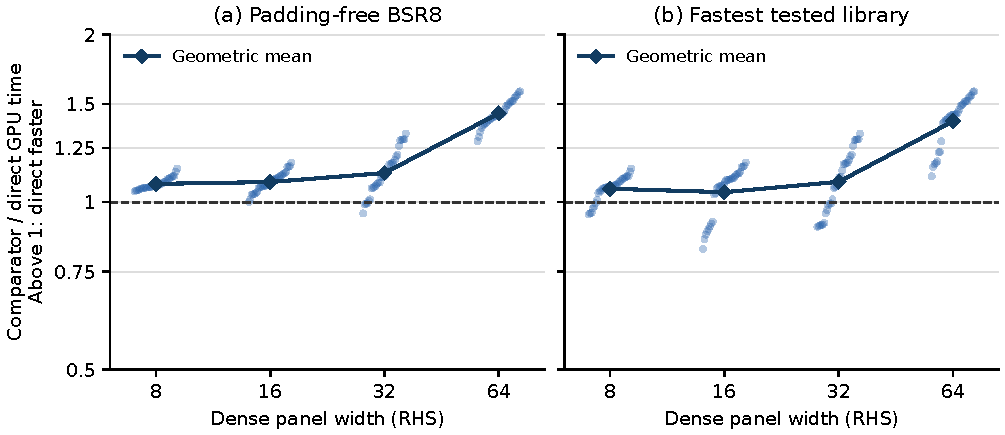
\includegraphics[width=\linewidth]{generated/use-cases.pdf}
\caption{Original core width comparison. Each point averages three
process ratios. The fastest-library panel uses the original NVIDIA controls.}
\end{figure}

\begin{table}[H]
\centering\small
\caption{Descriptive process-label ranges on the core grid. The two endpoints
are observed aggregate ratios, not confidence limits.}\label{tab:process}
\begin{tabular}{lrr}
\toprule
Comparator & Geometric mean & Process-label range \\
\midrule
CSR default & 4.932 & 4.893 to 4.979 \\
CSR lower envelope & 3.036 & 3.024 to 3.050 \\
Grouped cached & 4.129 & 4.116 to 4.153 \\
Grouped changing & 4.153 & 4.135 to 4.181 \\
\bottomrule
\end{tabular}

\end{table}

\begin{table}[H]
\centering\small
\caption{Width and degree breakdown for the core grid. Times are milliseconds
and speedups are dimensionless.}\label{tab:regimes}
\begin{tabular}{rrrrr}
\toprule
RHS & Degree & Direct ms & CSR ratio & Grouped ratio \\
\midrule
8 & 2 & 0.284 & 1.061 & 3.138 \\
8 & 4 & 0.551 & 1.391 & 3.356 \\
8 & 8 & 1.047 & 2.074 & 3.689 \\
8 & 16 & 2.049 & 1.034 & 3.965 \\
16 & 2 & 0.233 & 2.211 & 3.919 \\
16 & 4 & 0.403 & 2.555 & 4.679 \\
16 & 8 & 0.736 & 3.586 & 5.628 \\
16 & 16 & 1.451 & 2.941 & 5.901 \\
32 & 2 & 0.283 & 3.441 & 3.460 \\
32 & 4 & 0.508 & 3.647 & 4.098 \\
32 & 8 & 0.836 & 4.641 & 5.316 \\
32 & 16 & 1.584 & 5.293 & 5.766 \\
64 & 2 & 0.414 & 4.630 & 2.737 \\
64 & 4 & 0.726 & 5.159 & 3.445 \\
64 & 8 & 1.356 & 5.899 & 4.240 \\
64 & 16 & 2.685 & 6.360 & 4.375 \\
\bottomrule
\end{tabular}

\end{table}

\begin{table}[H]
\centering\small
\caption{Size and degree-pattern controls with random column locality. Each
row averages eight configurations and three process observations.}\label{tab:scaling}
\begin{tabular}{rlrrr}
\toprule
Block rows & Degree pattern & CSR ratio & Grouped ratio & CSR wins \\
\midrule
256 & 16 in every row & 2.019 & 4.538 & 8/8 \\
256 & 0, 1, 16, 16 & 1.277 & 4.065 & 4/8 \\
1024 & 16 in every row & 2.463 & 4.482 & 8/8 \\
1024 & 0, 1, 16, 16 & 2.877 & 4.140 & 8/8 \\
4096 & 16 in every row & 3.392 & 5.213 & 8/8 \\
4096 & 0, 1, 16, 16 & 3.963 & 4.655 & 8/8 \\
\bottomrule
\end{tabular}

\end{table}

\begin{table}[H]
\centering\small
\caption{Matched control time divided by changed-policy time. RHS-8
effects are geometric marginal contrasts over the other two factorial
choices. Minima and maxima first average three process ratios for each
fixed matrix instance. They are observed ranges, not confidence limits.}
\label{tab:matched}
\begin{tabular}{rlrrr}
\toprule
RHS & Change & Ratio & Min & Max \\
\midrule
8 & Eight-row mapping & 1.075 & 0.995 & 1.153 \\
8 & Two accumulators & 0.972 & 0.825 & 1.084 \\
8 & One CTA instead of two & 0.943 & 0.837 & 1.011 \\
8 & Full-panel staging & 1.472 & 1.120 & 1.966 \\
16 & Wider accumulation & 1.084 & 0.918 & 1.506 \\
16 & Cooperative staging & 1.406 & 1.102 & 1.897 \\
16 & Double buffering & 1.022 & 0.925 & 1.104 \\
16 & Full-panel staging & 2.271 & 1.866 & 2.997 \\
32 & Wider accumulation & 1.310 & 1.113 & 1.598 \\
32 & Cooperative staging & 1.414 & 1.205 & 1.770 \\
32 & Double buffering & 1.012 & 0.846 & 1.191 \\
64 & Wider accumulation & 1.379 & 1.217 & 1.731 \\
64 & Cooperative staging & 1.632 & 1.493 & 1.857 \\
64 & Double buffering & 0.801 & 0.661 & 0.924 \\
\bottomrule
\end{tabular}

\end{table}


\begin{figure}[H]
\centering
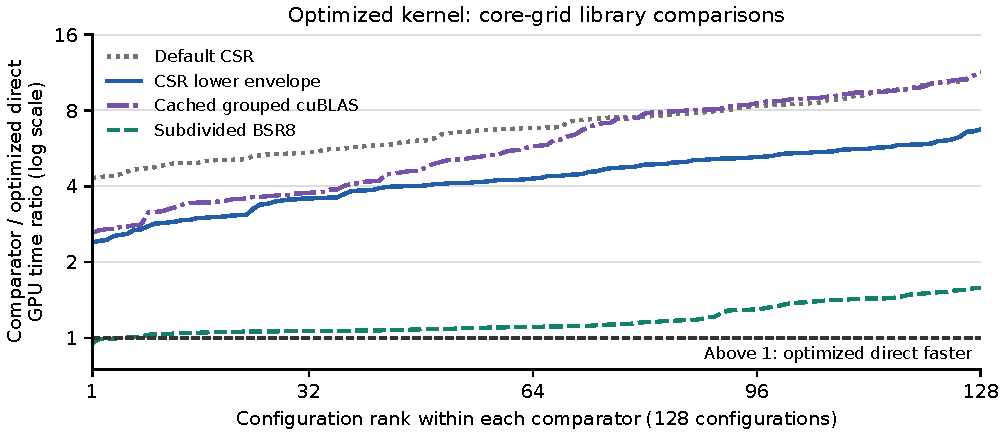
\includegraphics[width=\linewidth]{generated/core-distribution.pdf}
\caption{GPU time ratios across the 128 core configurations. Each ratio is
the geometric mean of three paired process ratios, computed from per-process
timing medians. Each curve sorts configurations independently, so equal ranks
need not identify the same matrix. The vertical axis is logarithmic. Ratios
above the dashed parity line favor direct execution. These are empirical
distributions over the chosen grid, not uncertainty intervals.}
\label{fig:core-distribution}
\end{figure}

\begin{table}[H]
\centering\small
\caption{All published-matrix controls, averaged across twelve matrix and
width configurations. Ratios divide comparator GPU time by direct time.}
\label{tab:application-controls}
\begin{tabular}{lrrr}
\toprule
Comparator & Ratio & Minimum & Direct wins \\
\midrule
Compact CSR & 0.352 & 0.210 & 0/12 \\
BSR8 & 0.648 & 0.498 & 0/12 \\
Grouped cached & 5.246 & 3.361 & 12/12 \\
Dense SGEMM & 1.051 & 0.460 & 7/12 \\
\bottomrule
\end{tabular}

\end{table}

\begin{table}[H]
\centering\small
\caption{Near-field comparator GPU time divided by direct time. Each row
averages three geometry seeds and three processes per seed. Ratios above
one favor direct execution.}\label{tab:native}
\begin{tabular}{rlrrrrr}
\toprule
Points & Geometry & RHS & CSR & BSR8 & Grouped & Dense \\
\midrule
2048 & uniform & 8 & 0.466 & 0.371 & 19.250 & 0.136 \\
2048 & uniform & 16 & 0.557 & 0.276 & 13.892 & 0.121 \\
2048 & uniform & 32 & 1.070 & 0.300 & 14.079 & 0.166 \\
2048 & uniform & 64 & 0.871 & 0.252 & 9.183 & 0.124 \\
2048 & clustered & 8 & 1.012 & 0.502 & 16.778 & 0.163 \\
2048 & clustered & 16 & 1.188 & 0.382 & 12.269 & 0.165 \\
2048 & clustered & 32 & 1.581 & 0.286 & 8.679 & 0.150 \\
2048 & clustered & 64 & 1.754 & 0.425 & 7.417 & 0.129 \\
8192 & uniform & 8 & 0.535 & 0.372 & 22.483 & 1.185 \\
8192 & uniform & 16 & 0.620 & 0.253 & 13.837 & 1.412 \\
8192 & uniform & 32 & 1.032 & 0.325 & 11.958 & 0.490 \\
8192 & uniform & 64 & 1.079 & 0.304 & 6.529 & 0.263 \\
8192 & clustered & 8 & 1.181 & 0.598 & 13.678 & 0.816 \\
8192 & clustered & 16 & 1.836 & 0.513 & 10.906 & 1.256 \\
8192 & clustered & 32 & 2.350 & 0.668 & 7.097 & 0.331 \\
8192 & clustered & 64 & 3.190 & 0.836 & 4.947 & 0.224 \\
\bottomrule
\end{tabular}

\end{table}
\FloatBarrier
\subsection{Core grid and format controls}
The original seed-1 campaign below uses three processes per configuration
and predates the MAGMA comparison. Its aggregates remain separate.
Table~\ref{tab:core} compares execution times on the core grid. The direct path has a
geometric speedup of \AuditCsr{} against the CSR lower envelope and
\AuditGrouped{} against cached grouped cuBLAS. The respective win counts
are \AuditCsrWins{} and \AuditGroupedWins{} out of 128 configurations.
Selecting the CSR algorithm reduces the aggregate ratio from
\AuditDefaultCsr{} for default CSR to \AuditCsr{} for the lower envelope.
The subdivided BSR8 ratio is \AuditBsrEight{}, with
\AuditBsrEightWins{} direct wins out of 128. This comparison retains block
structure without padding, comparing two ways to execute the same dense
blocks.
Figure~\ref{fig:core-distribution} shows the spread behind these averages.
Its sorted curves expose the fastest comparators and the width of the
performance range across the grid.



\begin{table}[H]
\centering\small
\caption{Core-grid ratios over 128 configurations and three process observations
per configuration. Minima and wins use GPU ratios averaged in log space across
processes. Changing-address grouped execution is paired with changing-address
direct execution.}\label{tab:core}
\begin{tabular}{lrrrr}
\toprule
Comparator & GPU ratio & Host ratio & Minimum & Wins \\
\midrule
CSR default & 4.932 & 4.856 & 1.655 & 128/128 \\
CSR lower envelope & 3.036 & 2.993 & 0.850 & 123/128 \\
Grouped cached & 4.129 & 4.077 & 2.606 & 128/128 \\
Grouped changing & 4.153 & 4.101 & 2.639 & 128/128 \\
\bottomrule
\end{tabular}

\end{table}



Table~\ref{tab:regimes} breaks down the same results by width and degree. Each row averages the four size distributions and two
localities. Direct time is the geometric mean of the corresponding process
medians. Absolute times distinguish small launch-sensitive cases from larger
products. The CSR column uses the lower envelope, and grouped execution uses
cached pointers.



\subsection{Additional seeds and queued comparisons}
The follow-up repeats all 128 core configurations on matrix seeds 2, 3,
and 5. Each seed and timing mode uses one fresh process per configuration,
giving 768 processes. The two modes synchronize after either one product
or eight queued products. Each process measures twenty samples, with GPU
and host times divided by the number of products in the sample. The eight
products use the same prepared plan and buffers. Changing-address controls
alternate the two buffer pairs on each product. Validation runs outside
timing, before and after the samples, and outputs are poisoned before each
method. Jobs and methods are randomized, and GPU processes run serially.

Table~\ref{tab:robustness} uses the same library lower envelope as the
original core comparison. Each row includes 32 configurations on each of
three matrix seeds. The seed range contains the smallest and largest
32-configuration geometric means. These ranges describe matrix variation
combined with process noise. There is one process for each seed and mode,
so they do not separate those sources or define confidence intervals.
The original three-process campaign remains separate. The follow-up uses
C++20 host compilation and the same library source bytes and CUDA toolkit.

\begin{table}[H]
\centering\small
\caption{Additional matrix seeds and synchronization intervals for the NVIDIA controls. Ratios divide
comparator time by direct time, so values above one favor direct execution.
Batch is the number of products queued before synchronization. Wins compare
direct execution with the fastest tested library for each of 96 instances.}
\label{tab:robustness}
\begin{tabular}{rrrrrr}
\toprule
Batch & RHS & Best library & BSR8 & Wins & Seed range \\
\midrule
1 & 8 & 1.056 & 1.081 & 75/96 & 1.052 to 1.060 \\
1 & 16 & 1.046 & 1.091 & 72/96 & 1.045 to 1.047 \\
1 & 32 & 1.091 & 1.131 & 65/96 & 1.087 to 1.094 \\
1 & 64 & 1.395 & 1.443 & 96/96 & 1.393 to 1.399 \\
8 & 8 & 1.050 & 1.074 & 73/96 & 1.049 to 1.052 \\
8 & 16 & 1.034 & 1.079 & 72/96 & 1.032 to 1.036 \\
8 & 32 & 1.086 & 1.125 & 64/96 & 1.075 to 1.104 \\
8 & 64 & 1.392 & 1.452 & 95/96 & 1.384 to 1.398 \\
\bottomrule
\end{tabular}

\end{table}

Across all 384 instances per mode, the fastest-NVIDIA-library ratios are
\RobustLatencyOverall{} for individual products and
\RobustQueuedOverall{} for batches of eight, with
\RobustLatencyWins{} and \RobustQueuedWins{} direct wins respectively.
Every width has a geometric-mean advantage on each additional seed in
both timing modes. RHS 64 gives the largest aggregate advantage, about
1.39, winning all 96 individual-product instances and 95 of 96 queued
instances. The narrow-panel gains remain smaller, about three to six
percent against the fastest tested library. Queueing eight products
preserves this width-dependent pattern on the measured grid.



\section{Transport discretization and follow-up controls}
For element width \(h\), the modal mass matrix has entries
\(M_{ii}=h/(2i+1)\). Set the characteristic displacement fraction to
\(\theta=\Delta t/h=1/4\). Exact translation followed by elementwise
\(L^2\) projection gives the stored one-step blocks
\[
 A^{\mathrm{self}}_{ij}=\frac{2i+1}{2}
 \int_{-1+2\theta}^{1}P_i(\xi)P_j(\xi-2\theta)\,d\xi,
\]
\[
 A^{\mathrm{upwind}}_{ij}=\frac{2i+1}{2}
 \int_{-1}^{-1+2\theta}P_i(\xi)P_j(\xi+2-2\theta)\,d\xi.
\]
The 96-point Gauss-Legendre rule integrates these polynomial products exactly
up to floating-point roundoff. Element orders repeat \(7,15,31,63\).
The block product retains each element's own basis and its upstream basis,
without scalar reblocking. This is a semi-Lagrangian DG update, replacing
the original forward-Euler experiment. Orthogonal projection after translation
is nonexpansive in physical \(L^2\) in exact arithmetic.

Initialization projects \(\sin(2\pi kx)\) for \(k=1,\ldots,N\).
All performance cases reach \(T=1/128\). Their 256, 1,024, and 4,096 elements
require 8, 32, and 128 products, respectively. Analytic comparisons project
\(\sin(2\pi k(x-T))\) and weight coefficient errors by \(h/(2i+1)\).
Every measured method checks its actual GPU result against that physical
reference as well as the independent repeated sparse-product reference.
An unchanged-state operation must fail the coefficient tolerances before
any timing starts. All six prepared inputs exceed a tenfold rejection
margin in both maximum absolute and relative coefficient error.

A separate FP64 spatial-refinement check keeps \(T=1/16\), the eight initial
waves, the repeating order schedule, and \(\theta=1/4\) fixed. With 16, 32,
and 64 elements, the analytic relative errors are
\(1.059\times10^{-6}\), \(6.253\times10^{-9}\), and
\(3.478\times10^{-11}\). The preparation script rejects a failure to reduce
error by at least a factor of four at each refinement. This is a smooth-wave
spatial-refinement check, not evidence for arbitrary nonlinear problems.
The FP64 check isolates discretization behavior from quantized FP32 arithmetic.

The trace comparator starts from identical prepared host blocks. Startup
includes method construction and one complete trace, including the reset
of its initial device buffer and output poisoning. Common panel allocations and Python assembly
are excluded. Every method's output is checked against repeated
FP64 sparse products using the assembled FP32 coefficients. No CPU reference
work occurs inside timing.

MAGMA slot execution needs no product workspace. The reduction composition
allocates \(64N\) FP32 entries per stored block. The alternating-buffer
transport trace retains two pointer plans and thus twice that product
workspace. The reduction kernel and all repeated slot calls are timed.
All MAGMA code is pinned in the source archive. This composition comparison
does not reproduce the full hierarchical solver from the motivating work.

\begin{table}[H]
\centering\small
\caption{Controlled combinations. Best-library-to-direct ratios average
three paired process ratios. Fixed-size 32 cases include BSR32.}
\begin{tabular}{rrrrrrrr}
\toprule
Rows & Degree & Size & RHS & Direct ms & BSR8 & MAGMA best & Best library\\
\midrule
128 & 4 & 8 & 8 & 0.013 & 1.398 & 1.299 & 0.916\\
128 & 4 & 32 & 8 & 0.016 & 0.853 & 1.769 & 0.853\\
128 & 4 & 8 & 64 & 0.015 & 0.799 & 2.297 & 0.799\\
128 & 4 & 32 & 64 & 0.025 & 1.277 & 1.863 & 0.961\\
128 & 16 & 8 & 8 & 0.025 & 0.527 & 1.001 & 0.527\\
128 & 16 & 32 & 8 & 0.043 & 0.795 & 1.221 & 0.795\\
128 & 16 & 8 & 64 & 0.034 & 0.458 & 1.874 & 0.458\\
128 & 16 & 32 & 64 & 0.074 & 1.272 & 1.719 & 0.985\\
128 & 128 & 8 & 8 & 0.138 & 0.364 & 1.031 & 0.364\\
128 & 128 & 32 & 8 & 0.496 & 0.681 & 0.724 & 0.681\\
128 & 128 & 8 & 64 & 0.191 & 0.338 & 2.407 & 0.338\\
128 & 128 & 32 & 64 & 0.643 & 1.088 & 1.783 & 0.792\\
512 & 4 & 8 & 8 & 0.016 & 0.694 & 1.848 & 0.618\\
512 & 4 & 32 & 8 & 0.024 & 1.157 & 2.254 & 0.981\\
512 & 4 & 8 & 64 & 0.034 & 0.450 & 1.705 & 0.450\\
512 & 4 & 32 & 64 & 0.070 & 1.252 & 1.825 & 0.932\\
512 & 16 & 8 & 8 & 0.031 & 0.483 & 2.204 & 0.483\\
512 & 16 & 32 & 8 & 0.080 & 1.221 & 2.213 & 0.902\\
512 & 16 & 8 & 64 & 0.109 & 0.278 & 2.080 & 0.278\\
512 & 16 & 32 & 64 & 0.315 & 1.207 & 1.677 & 0.842\\
512 & 128 & 8 & 8 & 0.193 & 0.314 & 2.743 & 0.314\\
512 & 128 & 32 & 8 & 0.673 & 1.075 & 2.130 & 1.043\\
512 & 128 & 8 & 64 & 0.808 & 0.224 & 2.285 & 0.224\\
512 & 128 & 32 & 64 & 2.388 & 1.406 & 1.783 & 1.112\\
\bottomrule
\end{tabular}

\end{table}

\paragraph{Update paths.} On the 256-block-row RHS-32 API test, value replacement plus execution takes 0.058 ms in synchronized host time, versus 0.213 ms for borrowing changed structure, validating its metadata, rebuilding the row order, and executing. These are geometric means of three process medians, with twenty samples each. Values alternate between two pre-existing device payloads on fixed degree-four structure. Structural cases alternate between degree-four and degree-eight matrices already on the GPU. Thus this is an API-path cost comparison, not an equal-work kernel speedup or a measurement of assembling a new structure.

\FloatBarrier
\section{Numerical behavior and input census}
Device sources are compiled with \texttt{-{}-use\_fast\_math}, which implies
\texttt{-ftz=true} (see the CUDA compiler reference in the main paper). Each output entry is a sum of products evaluated as
FP32 multiply-add with FP32 accumulation, in an unspecified order, with no
compensated summation. Flush-to-zero applies per instruction, to that
instruction's inputs and to its rounded result. It does not apply to the
product term inside a fused multiply-add, which is computed exactly and added
to the accumulator before a single rounding, so
\(\mathrm{fma}(\mathrm{FLT\_MIN},0.5,\mathrm{FLT\_MIN})\) retains
\(1.5\,\mathrm{FLT\_MIN}\). The consequences still cannot be excluded by
inspecting the caller's inputs. An instruction input, or an accumulator value
an instruction produces, that lands in the subnormal range is replaced by zero,
so contributions that pass through a subnormal accumulator are lost: two
contributions of \(\mathrm{FLT\_MIN}\times 0.5\) have normal operands and an
exact sum of \(\mathrm{FLT\_MIN}\), and the kernel returns zero at every
supported width, because each multiply-add produces a subnormal result from a
zero accumulator.
A partial sum above \(\mathrm{FLT\_MAX}\) becomes an infinity even when the
exact sum is finite, and the unspecified order means a later cancelling term
cannot be relied on. Accumulated error otherwise grows with the number of
terms and with cancellation, as in any uncompensated FP32 summation.

The claim is therefore verified rather than guaranteed. On the tested
workloads, results agree with a reference that accumulates in double and
rounds once, with maximum absolute error at most \(5\times10^{-4}\)
and relative L2 error at most \(5\times10^{-5}\). A dedicated range test pins
each behavior above, including the multi-contribution cases.

The measured inputs are not uniformly in the normal range. The three clustered
2,048-point covariance matrices contain 162, 212, and 294 subnormal packed
values. Those values carry less than \(10^{-30}\) of each matrix's total
magnitude, so their numerical contribution is negligible, and the measured
outputs pass the stated correctness checks. That is a statement about
numerical contribution, not about time: we did not measure these workloads
with and without flush-to-zero, so nothing here establishes that the timing
ratios are unaffected. A checked-in census keeps
these counts tied to the payloads. It covers the covariance and published
matrices and all six transport configurations, including the transport initial
states, references, and mass weights, which are operands as well. Those
contain no subnormal values.
\end{document}
